\documentclass[12pt,a4paper]{article}

\usepackage{fontspec}
\IfFontExistsTF{Times New Roman}
  {\setmainfont{Times New Roman}}
  {\IfFontExistsTF{CMU Serif}
    {\setmainfont{CMU Serif}}
    {\setmainfont{DejaVu Serif}}}
\IfFontExistsTF{Cascadia Mono}
  {\setmonofont{Cascadia Mono}}
  {\IfFontExistsTF{DejaVu Sans Mono}
    {\setmonofont{DejaVu Sans Mono}}
    {\setmonofont{CMU Typewriter Text}}}

\usepackage{geometry}
\geometry{left=25mm,right=15mm,top=20mm,bottom=20mm}
\setlength{\emergencystretch}{3em}
\usepackage{amsmath}
\usepackage{fvextra}
\usepackage{graphicx}
\usepackage{hyperref}
\hypersetup{hidelinks}

\title{Отчёт по задаче <<EFF\_k(alpha)>>}
\author{Смола Артём, группа 23.Б08}
\date{}

\begin{document}
\maketitle

\section{Постановка задачи}
Для КС-грамматики, параметра $k \ge 1$ и цепочки $\alpha$ требуется построить множество $EFF_k(\alpha)$:
\begin{enumerate}
    \item Рассмотреть терминальные цепочки, получаемые правосторонними выводами из $\alpha$.
    \item Для каждой цепочки взять всю цепочку при длине меньше $k$, иначе префикс длины $k$.
    \item Добавить результат в $EFF_k(\alpha)$ только если последнее правило вывода не является $\varepsilon$-продукцией.
\end{enumerate}

\section{Принцип решения}
Реализация строит правосторонние выводы из $\alpha$.
Состояние --- текущая сентенциальная форма.
На каждом шаге раскрывается только правый нетерминал.

Для каждого терминального листа:
\begin{itemize}
    \item добавляется префикс в множество \texttt{ALL\_PREFIXES};
    \item в \texttt{EFF} добавляется только если последнее правило имеет непустую правую часть.
\end{itemize}

Для защиты от бесконечного роста вывода используются ограничения
\texttt{max\_nodes} и \texttt{max\_form\_chars}.

\section{Корректность}
На каждом шаге раскрывается именно правый нетерминал, поэтому рассматриваются только правосторонние выводы.
Для каждого терминального листа формируется префикс длины $\min(|w|, k)$, что совпадает с определением $EFF_k$.
Фильтр по непустой правой части последнего правила точно реализует условие
``последнее правило не $\varepsilon$-продукция''.
Следовательно, множество \texttt{EFF} в программе совпадает с требуемым $EFF_k(\alpha)$.

\section{Ограничения реализации}
\begin{itemize}
    \item для защиты от бесконечных выводов используются лимиты на число узлов и длину формы;
    \item при срабатывании лимитов печатается предупреждение, а вывод может быть неполным;
    \item в расширенном формате символы должны входить в объявленные множества нетерминалов и терминалов.
\end{itemize}

\section{Исходный код}
Исходный код программы и тестовые данные доступны в репозитории GitHub:
\url{https://github.com/artem-smola/formal_lang}.

\section{Код программы}

Код программы:

{\small
\VerbatimInput[
    fontsize=\footnotesize,
    breaklines=true,
    breakanywhere=true
]{../../Code/main.cpp}
}

\section{Демонстрация работы программы}
\subsection*{1) Входные данные}
\textbf{Рассматриваемый тест:} \texttt{test1}.

Формат входных данных:
\begin{enumerate}
    \item Поддерживаются краткий и расширенный режимы ввода.
    \item В кратком режиме задаётся $k$, затем продукции и цепочка $\alpha$.
    \item В расширенном режиме используются директивы \texttt{k}, \texttt{start},
    \texttt{nonterminals}, \texttt{terminals}, строки \texttt{alpha} и продукции.
    \item В обоих режимах можно задать \texttt{max\_nodes} и \texttt{max\_form\_chars}.
\end{enumerate}

Нетерминалы --- символы $A..Z$.
Пустая альтернатива, \texttt{eps} или \texttt{epsilon} задают $\varepsilon$-продукцию.

{\small
\VerbatimInput[
    fontsize=\footnotesize,
    breaklines=true,
    breakanywhere=true
]{../../Code/tests/test1.in}
}

\subsection*{2) Вывод}

\begin{center}
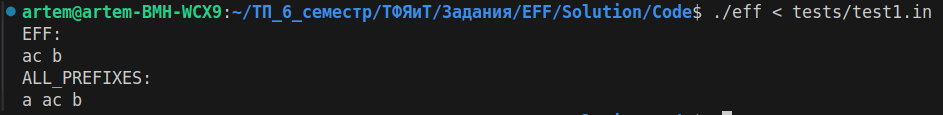
\includegraphics[
    width=\textwidth,
    keepaspectratio
]{assets/output.png}
\end{center}

\subsection*{3) Визуализация}
\IfFileExists{../../Visualization/test1.png}{
\begin{center}

\includegraphics[
    width=\textwidth,
    height=0.40\textheight,
    keepaspectratio
]{../../Visualization/test1.png}
\end{center}
}{
\textbf{Файл визуализации:} \texttt{../../Visualization/test1.dot}

{\small
\VerbatimInput[
    fontsize=\footnotesize,
    breaklines=true,
    breakanywhere=true
]{../../Visualization/test1.dot}
}
}

\subsection*{4) Описание результата}
Для теста \texttt{test1} получено:
\begin{itemize}
    \item \texttt{EFF = \{ac, b\}};
    \item \texttt{ALL\_PREFIXES = \{a, ac, b\}}.
\end{itemize}
Цепочка \texttt{a} присутствует в \texttt{ALL\_PREFIXES}, но отсутствует в \texttt{EFF}.
Причина в том, что она получена веткой, где последнее применённое правило --- $\varepsilon$-продукция.
Этот пример показывает, почему \texttt{ALL\_PREFIXES} может быть строго больше \texttt{EFF}.

\subsection*{5) Дополнительный граничный тест}
Для \texttt{test3} получается пустое слово в \texttt{ALL\_PREFIXES}:

\textbf{Входные данные теста \texttt{test3}:}

{\small
\VerbatimInput[
    fontsize=\footnotesize,
    breaklines=true,
    breakanywhere=true
]{../../Code/tests/test3.in}
}

\[
\mathrm{ALL\_PREFIXES} = \{\varepsilon, c, d\},\qquad
\mathrm{EFF} = \{c\}.
\]
Это демонстрирует фильтрацию финальной $\varepsilon$-ветви и корректную обработку пустой цепочки.

\section{Анализ сложности}
Пусть:
\begin{itemize}
    \item $M$ --- число реально раскрытых сентенциальных форм;
    \item $R$ --- среднее число продукций для раскрываемого нетерминала;
    \item $L$ --- средняя длина формы.
\end{itemize}

Тогда время:
\[
O(M \cdot R \cdot L),
\]
так как каждый переход строит новую форму заменой правого нетерминала.

Память:
\[
O(M \cdot L),
\]
на хранимые формы в стеке и в множестве уже раскрытых состояний.

\end{document}
